\newpage

\section{Implementation}
The WALE model has been implemented initially in the D3Q27 Matrix LBM solver~\cite{sonja:12} developed in the Institute of Computational modelling in Civil Engineering (iRMB). This code uses two set of arrays to store the distribution functions. The WALE model implementation requires the computation of the strain rate tensor and the vorticity rate tensor, which requires the information of the velocity gradients. The velocity gradients have been computed using the finite differences. The macroscopic velocities computed from the distribution functions are used to compute the velocity gradients in every time-step. Apart from the WALE model implementation the topic on the conditioning of the WALE model equation will be discussed here. Towards the end of the section the numerical results of the Taylor green vortex simulations will be compared to the analytical solution to confirm the validity of the order of of the eddy-viscosity obtained from the WALE model.

\subsection{Discretisation}
Several velocity gradients i.e. $\partial u_i/\partial x_i$ and $\left(\partial u_i/\partial x_j + \partial u_j/\partial x_i\right)$ are directly available from the Cumulant LB solver~\cite{geier:parameter}. The computation of the strain rate tensor can be easily carried out with those available gradients. But the available information of the velocity gradients was not enough to compute the rotation rate tensor i.e. $\left(\partial u_i/\partial x_j - \partial u_j/\partial x_i\right)$. Since the vorticity calculations had to be  performed using the finite difference method, it was decided to compute the velocity gardients using the finite difference method. \emph{Weickert et.al}~\cite{weickert:LES} implemented the WALE model in the MRT LB framework and they have computed the velocity gradients using the finite differences. 

The purpose of the SGS models is to dissipate the resolved turbulent fluctuations~\cite{davidson}. When finite differences are used in combination with the LES method great care has to be taken to choose the non-dissipative finite difference scheme. This is done to avoid the masking effect of the numerical dissipation on to the dissipation introduced by the SGS models. Taking that into consideration a central difference scheme was chosen to compute the velocity gradients.\\\\
%
\textbf{Treatment of velocity gradients near the boundaries}

In order to avoid the fluid nodes, near the boundaries, accessing the non-fluid nodes due to the central differencing, forward differences and backward differences were used at the respective boundaries to compute the velocity gradients. Fig.(\ref{Finite differences bound}) shows a cuboid marked with the red dots at the inlet, front and the bottom face. The first set of fluid nodes near these faces use forward difference to compute the velocity gradients and the first set of fluid nodes at the exit, top and back faces use backward differences to compute the gradients along the respective directions. Rest fluid nodes used central differences.

\begin{figure}[t]
\centering
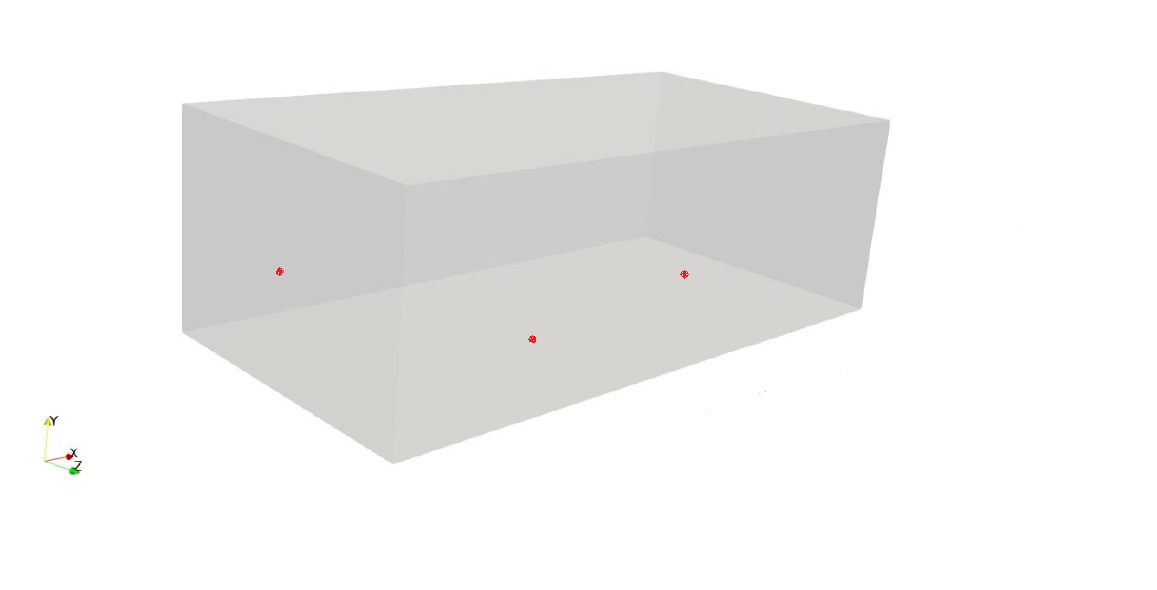
\includegraphics[width=8cm]{04_Implementation/figur/3D_Domain_gradients.png}
\label{Finite differences bound}
\caption{Cuboid representing a channel}
\end{figure}
\subsection{Implementation of eddy viscosity contribution}

The WALE model has been implemented in the LB kernel itself "LB\_Kernel\_2SOD". Few other variations were tried but they required thread synchronisation which is not optimal to do in terms of the efficiency. Hence, it was implemented in the kernel itself. An additional viscosity called eddy viscosity $\left(\nu_t\right)$ has to be introduced in to the solver to model the turbulence. This is given by:
%
\begin{equation}
\label{Eddy viscosity}
\nu_t = \left(C_W \Delta_x \right)^2 \overline{OP}
\end{equation}
%
where $C_W$ is the model constant and $C_W = 0.5 $ as mentioned in the \emph{Nicoud et.al}~\cite{nicoud:WALE}. In this LBM-LES investigation we will be using the implicit filtering, where the filter size is proportional to the grid size. The filter size $\Delta_x = 1$ is taken since we have a uniform lattice and a uniform mesh. \\
The total viscosity is the summation of the molecular viscosity and the eddy viscosity:
%
\begin{equation}
\label{Total viscosity}
\nu_{total} = \nu + \nu_t
\end{equation}
%
The total viscosity and the total relaxation time are related by ~\cite{weickert:LES} :
%
\begin{equation}
\label{Total rel. time}
\tau_{total} = 3\nu_{total} + \frac{1}{2}
\end{equation}
%
The value of $\nu$ is provided as the input to the solver and the $\nu_t$ is computed in the solver. To compute $\nu_t$ the eq.(\ref{traceless tensor-1}) \& eq.(\ref{eddy-viscosity}) are used. Now the relaxation parameter responsible to include the transport properties in the solver is $s9$ and it is related to the total relaxation time as follows:
%
\begin{equation}
\label{s9}
s9 = \frac{1}{\tau_{total}}
\end{equation}
%
\subsubsection{Conditioning of the WALE model equation}

In order to perform the initial tests of the implementation an in-built case in the D3Q27 Matrix solver was used. It is a 3D case with a cube placed in the channel. These tests were to get a feeling whether the implementation is working properly or not. No comparison or any such investigation was performed with the test case. Thus, no results of the tests will be presented. It is has been mentioned here for the sake of completion.

When performing such tests it was found that the solver generated "NaN" (Not a number) in the output. After examining the individual resulting quantities viz. all terms in the eq.(\ref{eddy-viscosity}), $\tau_{total}$ etc. It was observed that for certain initial time-steps the numerator and the denominator of the eq.(\ref{eddy-viscosity}) were becoming zero and eventually it resulted in the mathematical error of the form $\frac{0}{0}$.\\
This issue was resolved by adding a small number in the denominator of the eq.(\ref{eddy-viscosity}). Till now the implementation and the tests were performed using the single precision on the local machine equipped with GeForce GTX 760. The small parameter $\left(\epsilon\right)$ of the order $10^{-10}$ was added in the numerator and this resolved the issue of the ill-conditioned equation. The resulting eddy viscosity looks like:
%
\begin{equation}
\label{mod eddy visc}
\begin{split}
{\nu_t} &= \left({C_w}{\Delta}\right)^{2} \frac{\left({S_{ij}^{d}}{S_{ij}^{d}}\right)^{3/2}}{\left(\sij \sij\right)^{5/2} + {\left({S_{ij}^{d}}{S_{ij}^{d}}\right)^{5/4}} + \epsilon} 
\end{split}
\end{equation}
%

Once the model started to work it was then fitted into more efficient implementation of Cumulant LB solver. 
\subsection{Taylor-Green vortex simulations (TGV)}

Once the implementation was fitted in the new code it was tested for the case of turbulent channel flow (see section \ref{validation}). It was observed that the resulting $\nu_t$ was very small i.e. of order $10^{-11}$ for single precision. Several options were tried, but it was difficult to narrow down the cause for it. 

Hence it was decided to perform the Taylor-Green vortex~\cite{taylor:green} simulation. The TGV is an unsteady flow of a decaying vortex, which has an exact closed form solution of the incompressible Navier–Stokes equations in Cartesian coordinates~\cite{wiki:tgv}. Since we know the analytical solution of this simple flow, in comparison to the three dimensional turbulent channel flow, this case was chosen to verify the WALE model implementation for the $\nu_t$
%compare the numerically computed eddy viscosity with the analytical one. 

\subsubsection{Simulation settings}

A rectangular computational domain has been chosen to perform the TGV simulation. The aspect ratio of the domain, $h/l$, is chosen to be: $1.2$. The domain is of Quasi 3D type as we want to perform two-dimensional TGV simulation. This is done as any three dimensional LB solver cannot simulate 2D flows. The input physical quantities and the output are in Lattice Boltzmann units. The width of the domain, in y-direction, is $4\Delta x$. 

A hierarchy of three meshes have been generated to see the effect of resolution on to the $\nu_t$. The resolution for length i.e. along the x-coordinate direction varies from $32\Delta x$ to $128\Delta x$ and the resolution for the height i.e. along the z-coordinate direction varies from $48\Delta x$ to $192\Delta x$. All faces of the Quasi 3D domain are assigned with periodic boundaries.
The equations used for the initialisation have been specified as follows:
%
\begin{equation}
\label{TGV den}
\rho\left(t=0\right) = \frac{3}{4} U^2 \left(cos\left(x\right)\frac{4\pi}{L_x} + cos\left(z\right)\frac{4\pi}{L_z}\right)\frac{L_z}{L_x}\\
\end{equation}
%
%
\begin{equation}
\label{TGV u}
u\left(t=0\right) = U\ sin\left(x\right)\frac{2\pi}{L_x}\ cos\left(z\right)\frac{2\pi}{L_z}\\
\end{equation}
%
%
\begin{equation}
\label{TGV w}
w\left(t=0\right) = U\ cos\left(x\right)\frac{2\pi}{L_x}\ sin\left(z\right)\frac{2\pi}{L_z}\\
\end{equation}
%
%
\begin{equation}
\label{TGV v}
v\left(t=0\right) = 0\\
\end{equation}
%
where $U \Delta x / \Delta t$ is the initial velocity scale and $L_x$, $L_z$ are respectively the length and the height of the domain. The table (\ref{resolution TGV}) shows the different mesh resolutions along with the $U$ for different mesh resolutions. The value of the kinematic viscosity was taken as $\nu = 10^{-4} m^2/s$. The viscosity is kept fixed and the resolution along with the $U$ are varied to have the same Reynolds number for all mesh resolutions. 
%
\begin{table}[h!]
\begin{center}
\begin{tabular}{ p{1.5cm}|p{2.5cm}|p{1cm}} 

 & $N_x$ x $N_y$ x $N_z$ & $U$\\
  \hline
   Mesh 1& 32 x 4 x 48 & 0.1\\
  \hline
  Mesh 2& 64 x 4 x 96 & 0.05\\
  \hline
  Mesh 3 & 128 x 4 x 192 & 0.025\\
  \hline
\end{tabular}
\end{center}
\caption{Mesh resolution used in TGV simulations}
\label{resolution TGV}
\end{table}
%
\subsubsection{Analytical settings}
Using the analytical solution equations of the incompressible Navier-Stokes equation for the TGV and the WALE model the analytical $\nu_t$ can be obtained. The WALE model was implemented in MATLAB for computing the analytical $\nu_t$. The paramters shown in table (\ref{resolution TGV}) are also applicable here. The two dimensional analytical solution equations~\cite{krueger:book} are as follows:
%
\begin{equation}
\label{analytical sol}
\begin{split}
u &= U \sqrt{\frac{k_x}{k_z}}sin\left(k_xx\right)cos\left(k_zz\right)e^{-\frac{t}{t_d}}\\
w &= U \sqrt{\frac{k_z}{k_x}}cos\left(k_xx\right)sin\left(k_zz\right)e^{-\frac{t}{t_d}}\end{split}
\end{equation}
%
where $k_x = 2\pi/L_x$ and $k_z = 2\pi/L_z$. The term $t$ is the total simulation time and the $t_d = 1/\nu\left(k_x^2 + k_z^2\right)$ is the decay time of the vortex.

While computing the analytical value of $\nu_t$ it was observed that the terms in the numerator and denominator of eq.(\ref{mod eddy visc}) were very small, order $10^{-15}$ to $10^{-25}$ compared to the value of $\epsilon$ added. This was the reason for not getting the correct values of $\nu_t$. Thus the value of $\epsilon$ was set to $10^{-30}$ for single precision.

\subsubsection{Results \& comparison}

In this subsection the numerically and analytically computed TGV results obtained with the changed value of $\epsilon$ is presented. The table(\ref{solver TGV}) shows the number of time-steps, $N_t$, for which the simulation of each resolution was run and the time interval, $\Delta t$ for writing out the results. With the increase in the resolution, the simulations were also run for a longer time. The factor with which the resolution changes is same as the factor of increase in the $N_t$.

%
\begin{table}[h!]
\begin{center}
\begin{tabular}{ p{1.5cm}|p{2.5cm}|p{1cm}} 

 & Time-steps, $N_t$ & $\Delta t$\\
  \hline
   Mesh 1& 4000 & 100\\
  \hline
  Mesh 2& 8000& 200\\
  \hline
  Mesh 3 & 16000 & 400\\
  \hline
\end{tabular}
\end{center}
\caption{Solver settings for TGV}
\label{solver TGV}
\end{table}
%

%
\begin{figure}[h]
%\centering
\begin{minipage}[b]{0.5\textwidth}
\subfigure[global coordinates]{
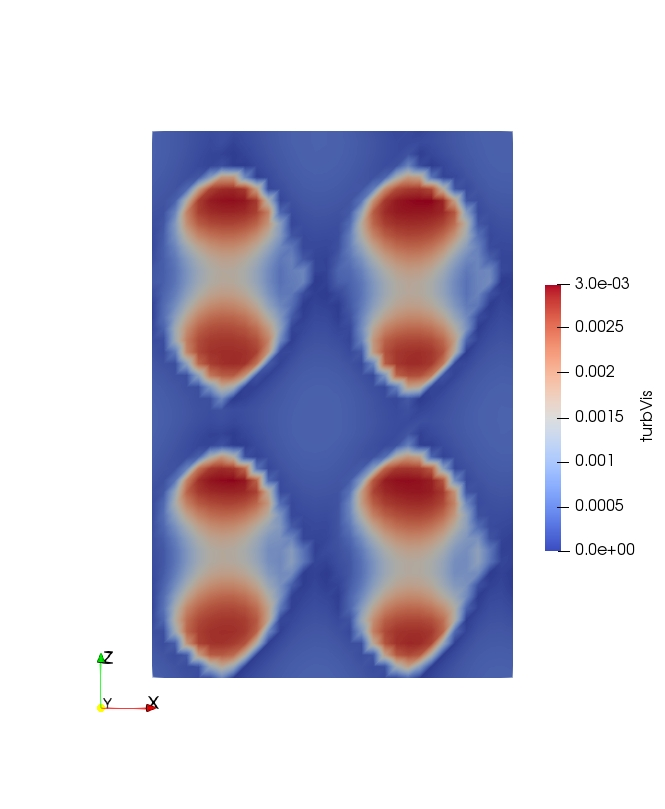
\includegraphics[width=6.7cm]{04_Implementation/figur/nutSimulation_change.jpg}}
\end{minipage}
%
\begin{minipage}[b]{0.5\textwidth}
\subfigure[global coordinates]{
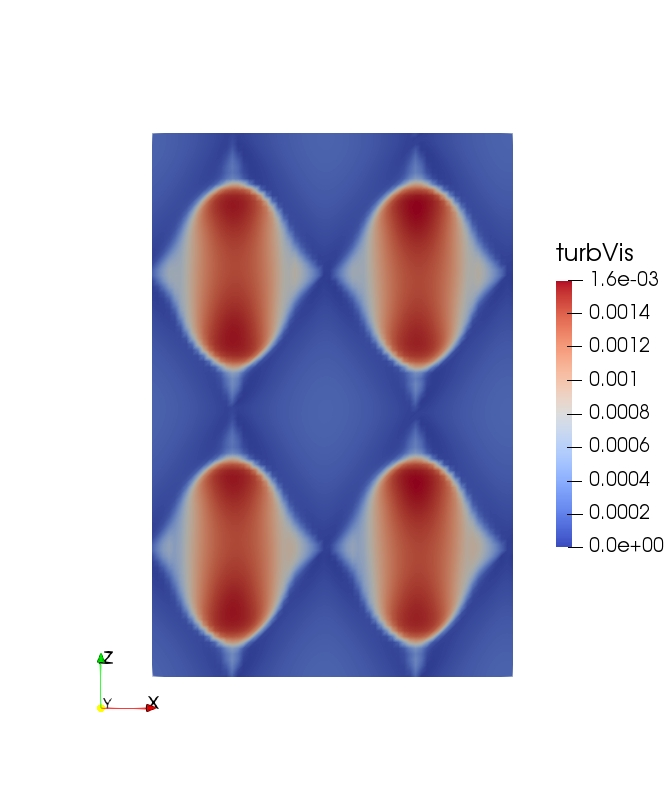
\includegraphics[width=6.7cm]{04_Implementation/figur/nutSimulation_latex_64.jpg}}
\end{minipage}
\end{figure}
%

%
\begin{figure}[h]
%\centering
\begin{minipage}[b]{0.5\textwidth}
\subfigure[global coordinates]{
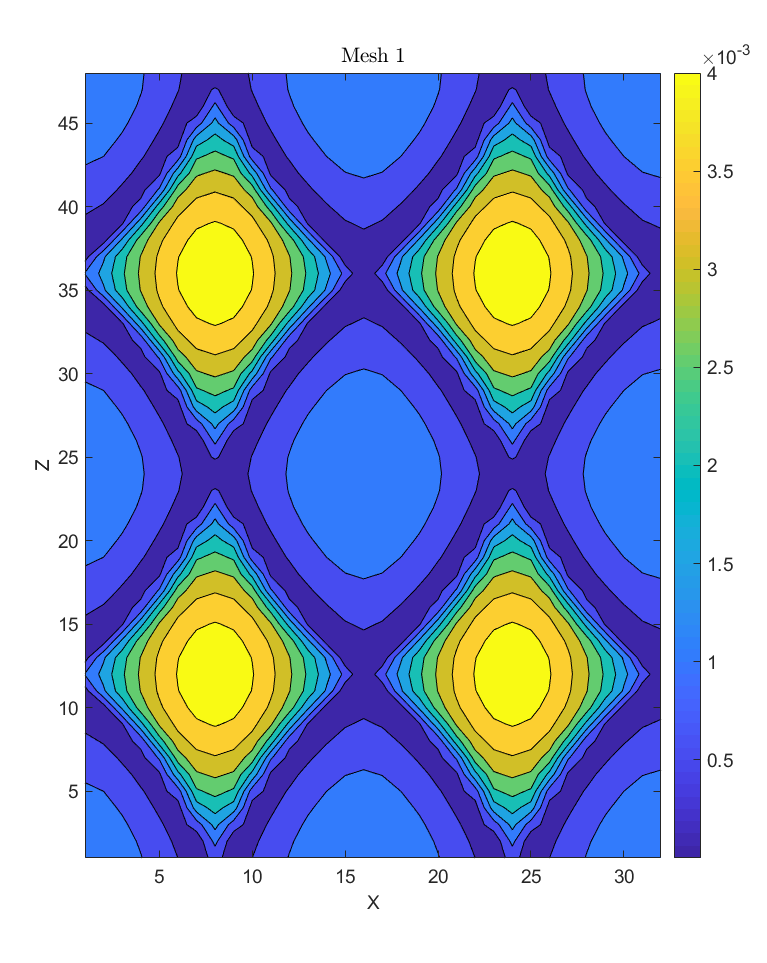
\includegraphics[width=6.7cm]{04_Implementation/figur/nut_32x4x48.png}}
\end{minipage}
%
\begin{minipage}[b]{0.5\textwidth}
\subfigure[global coordinates]{
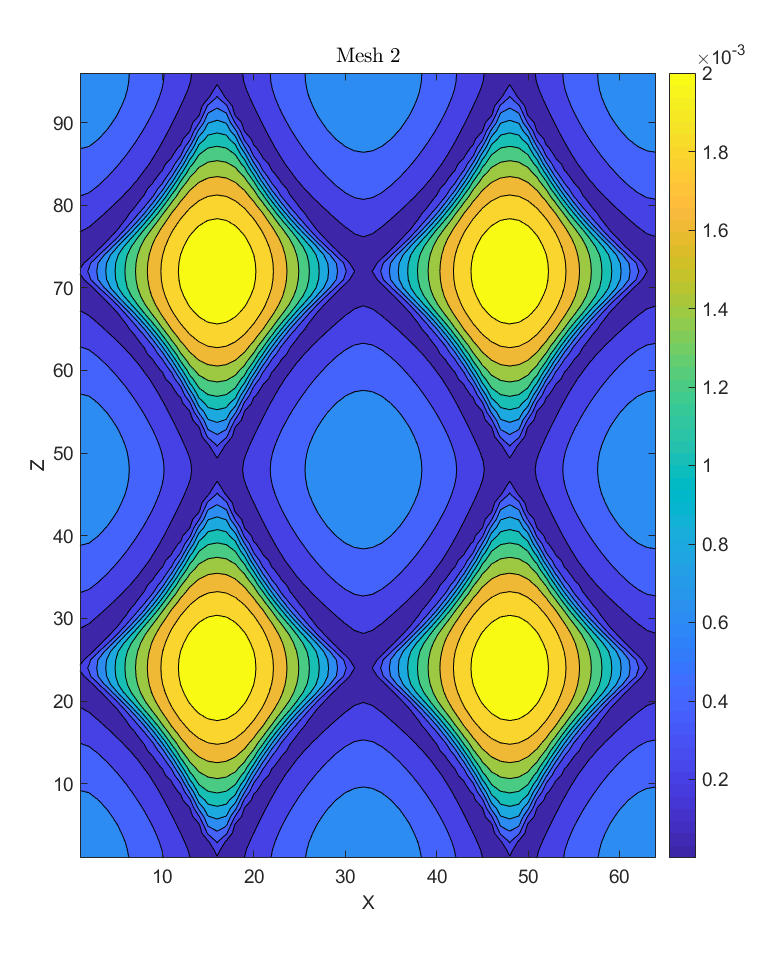
\includegraphics[width=6.9cm]{04_Implementation/figur/nut_64_half.png}}
\end{minipage}
\end{figure}
%

